

\chapter{Introduction}

%\narrowlinespacing
%\begin{myquote}
%\begin{flushright}
%\textit{Creativity is knowing how to hide your sources.} \\-- Cyril Edwin Mitchinson Joad
%\end{flushright}
%\end{myquote}
%\normallinespacing

\section{Anatomy of a movement: Muscle} %breakdown
Performing a locomotion task is a complicated process that involves many physiological entities working in high coherence. It involves bones, tendons, nerves, and many other systems working in perfect harmony, from basic cellular and electrochemical level to highest organizational levels of the organism. Even the simplest movements are rarely performed using just one muscle. Everything we do involves high muscular coordination and constant and precise regulation. While standing, for example, muscles of the legs and the trunk are constantly simultaneously co-contracting, maintaining balance.  

The neural system has an important controlling function, but the actual force required to perform a movement is generated in the muscles. A muscle is a body tissue capable of transforming chemical energy to force. There are several muscle types: smooth, building internal organs, cardiac, building the heart, and skeletal. Only skeletal muscles can be controlled voluntarily and are used in locomotion. They are usually connected to bones with tendons (collagen fibers).

The neurons controlling the movement are organized in a hierarchical fashion \citep{Widmaier2014}. In the highest level of hierarchy, a movement is conceived. Very little is known about the exact location of neurons and brain centers responsible for this task. These centers transmit the command to the middle level structures, where the task is elaborated. Simultaneously, these middle level neurons receive the information from the receptors in muscles, skin, tendons, and joints, but also from the visual system. All this information is taken into account when deriving a movement. Planning of the movement that is about to be executed is performed with respect to the space this movement will occupy, and control signals for each muscle involved in the movement are generated. The centers involved in these tasks are located in the cerebral cortex, the cerebellum, the subcortical nuclei, and the brain stem. The information is then transmitted to the lowest level of the motor hierarchy: the spinal cord and the brain stem. At this level the information is transmitted through the motor neurons to the muscles. The selection of the exact motor neurons and the exact timings of their activations are planned. The organization and the locations of the neural system for motor control can be seen in figure \ref{fig:brain_centers}, whereas the overall figure of motor control can be seen in figure \ref{fig:control-merletti}.
\begin{figure*}[t!]
    \centering
    \begin{subfigure}[t]{0.95\textwidth}
        \centering
        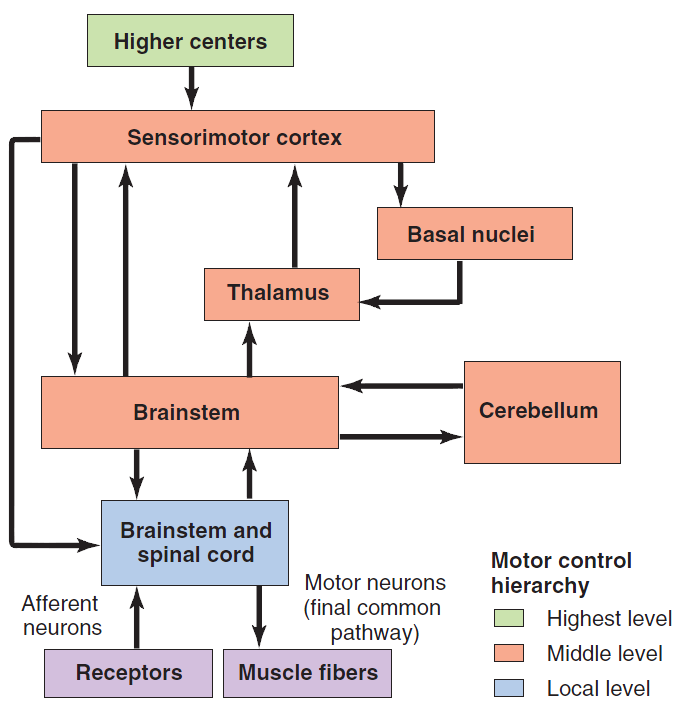
\includegraphics[height=3in]{Images/introduction/control.png}
        \caption{}
    \end{subfigure}%
    
    \begin{subfigure}[t]{0.95\textwidth}
        \centering
        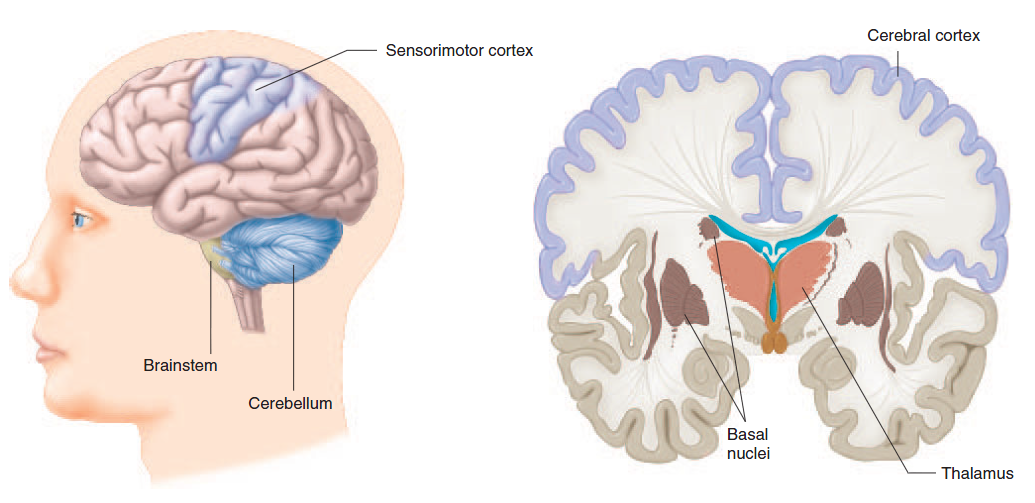
\includegraphics[height=3in]{Images/introduction/control2.png}
        \caption{}
    \end{subfigure}
    \caption{Figure describes \textbf{a)} hierarchical organization of the neural system for motor control and \textbf{b)} side view and cross section of the brain showing motor control centers. Retrieved from \citet{Widmaier2014}.}
\label{fig:brain_centers}
\end{figure*}

\begin{figure}[ht]
\centering
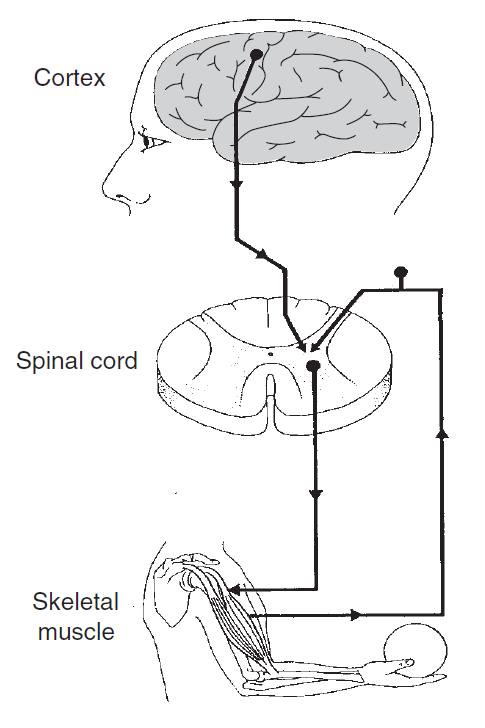
\includegraphics[width=0.45\textwidth]{Images/introduction/control-merletti2.png}
\caption{Figure represents a schematic representation of the motor control mechanisms. Idea of a movement is conceived in the brain, and is getting to the spinal cord by neural pathways. Motor neurons exiting the spinal cord activate muscle contraction. Simultaneously, sensory information is being transmitted to the higher controlling mechanisms. Retrieved from \citet{Merletti-book}.}
\label{fig:control-merletti}
\end{figure}


\subsection{Muscle physiology}

The elementary building block of a muscle is a muscle cell, or a muscle fiber - \emph{myocyte}. Each myocyte is ensheated by \emph{endomysium}, a connective tissue that contains nerves and capillaries. Myocytes are organized in bundles of ten to hundred fibers, which are called \emph{fascicles}, and they are surrounded by a sheath of connective tissue, \emph{perymisium}. A group of fascicles is finally grouped together and enveloped by connective tissue, \emph{epimysium}, forming a muscle. Cross-section of a muscle can be seen in figure \ref{fig:muscle}.
\begin{figure*}[t!]
    \centering
    \begin{subfigure}[t]{0.49\textwidth}
        \centering
        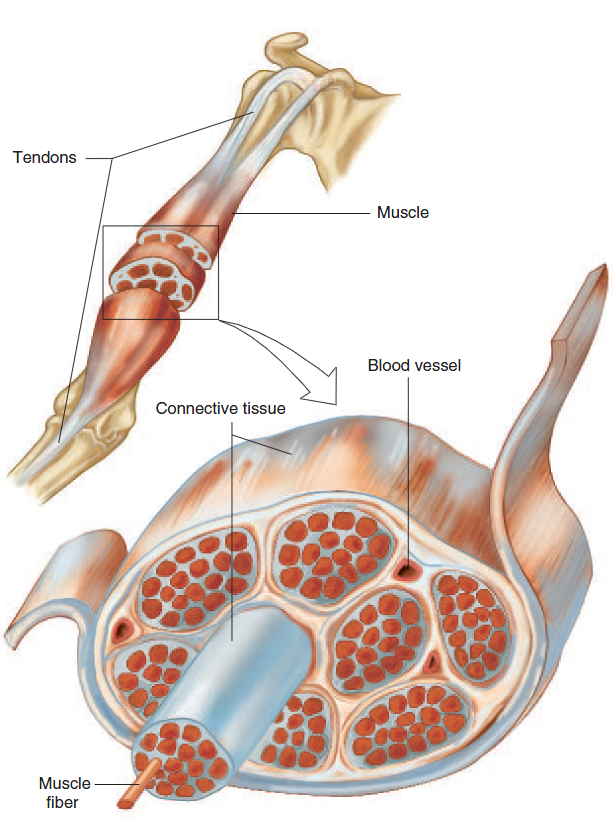
\includegraphics[height=4in]{Images/introduction/muscle.png}
        \caption{Retrieved from \citet{Widmaier2014}.}
    \end{subfigure}%
    ~ 
    \begin{subfigure}[t]{0.49\textwidth}
        \centering
        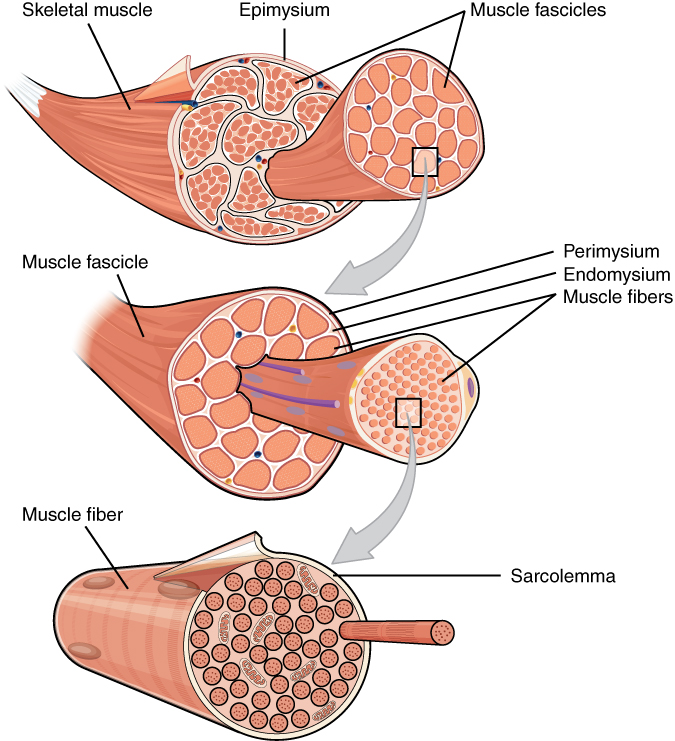
\includegraphics[height=3.4in]{Images/introduction/Muscle_Fibers.png}
        \caption{Retrieved from \citet{OpenStax2013}.}
    \end{subfigure}
    \caption{Figure shows \textbf{a)} cross-section of a skeletal muscle with attachment to a bone, and \textbf{a)} a detailed cross-section of a skeletal muscle from myofibrils to the entire muscle.}
\label{fig:muscle}
\end{figure*}
%\begin{figure}[ht]
%\centering
%\includegraphics[width=0.9\textwidth]{Images/introduction/Musle_Fiber.png}
%\caption{Organization of skeletal muscle with attachment to the bone. Retrieved from \citep{Widmaier2014}}
%\label{fig:muscle}
%\end{figure}

\emph{Sarcolema} is the cell membrane of a myocyte, consisting of a lipid bilayer that contains intracelular liquid, \emph{myoplasma}. In the myoplasma, thin and thick filaments are serially connected, forming \emph{sarcomeres}, which are longitudinally connected in \emph{myofibrils} that extend through entire length of the myocyte. During the shortening of muscle fibers, thin and thick filaments of sarcomeres are pulled together by cross-bridges between them. Total shortening of a myofibril is the summation of shortenings of sarcomeres of which it is composed.

Each motor neuron at the neuromuscular junction innervates several muscle fibers, forming the smallest functional unit called \emph{motor unit}. It was firstly defined by Liddell and Sherrington in 1925 \citep{Liddell1925, Sherrington1925} and is composed of a motor neuron with axon and dendrites, and muscle fibers that the axon innervates, as seen in the figure \ref{fig:motor units} \citep{Duchateau2011}. Since a motor neuron with a single action potential usually evokes action potentials simultaneously in all belonging muscle fibers, by observing the action potentials of the muscle fibers, information on activity of the motor neurons in the spinal cord or the brain stem can be inferred \citep{Merletti-Farina-book}. However, muscle fibers belonging to the same motor neuron are not grouped together within a muscle, but are intermingled with muscle fibers belonging to other motor units (see figure \ref{fig:motor units}b). The pool of motor neurons that innervates an entire muscle generally ranges from ten to a thousand, depending on the muscle \citep{Merletti-Farina-book}. Muscles controlled by a higher number of motor neurons can achieve finer and more precise movements, e.g. hand movements.
\begin{figure*}[t!]
    \centering
    \begin{subfigure}[t]{0.49\textwidth}
        \centering
        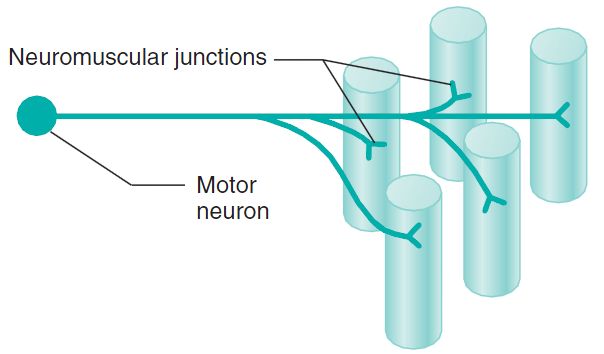
\includegraphics[height=1.7in]{Images/introduction/one_MU.png}
        \caption{}
    \end{subfigure}%
    ~ 
    \begin{subfigure}[t]{0.49\textwidth}
        \centering
        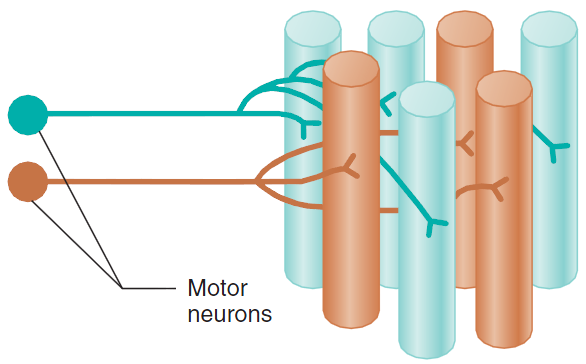
\includegraphics[height=1.7in]{Images/introduction/two_MU.png}
        \caption{}
    \end{subfigure}
    \caption{Figure shows \textbf{a)} a single motor unit with motoneuron and muscle fibers it innervates, and \textbf{b)} two motor units. It can be seen that muscle fibers of different motor units are intermingled. Retrieved from \citet{Widmaier2014}.}
\label{fig:motor units}
\end{figure*}


By the characteristics of a muscle fiber, there are three main types of muscle fibers:
\begin{description}
\item[Fast twitch, fatigable fibers (FF, or type IIb):] These fibers have high levels of ATP (source of energy) for anaerobic energy supply, and are dominantly present in pale muscles. They are of glycolytic type and work well in ischemic or low oxygen conditions. Regarding contraction properties, they are characterized by a fast twitch, large forces, and a high nerve conduction velocity, but they get fatigued faster than the other muscle fiber types. 

\item[Fast twitch, fatigue-resistant (FR, or type IIa):] These are oxidative glycolytic fibers, characterized by a fast twitch and are resistant to fatigue. They have an intermediate conduction velocity. 

\item[Slow twitch, very resistant to fatigue (S, or type I):] They are slow oxidative fibers and do not work well in low oxygen conditions. They generate small forces, have a slow twitch, and are characterized by a lower nerve conduction velocity. This fiber type is very resilient to fatigue because of the high oxidative metabolism and energy efficiency. They are present in a high percentage in red muscles, such as soleus.
\end{description}

Muscle fibers innervated by the same motor neuron have similar histochemical and contractile characteristics, and can be said that a motor unit is composed of muscle fibers of the same type \citep{Merletti-book}.


A force that muscle fibers generate depends on the firing frequency of the action potentials innervating the neuromuscular junction (rate coding), and the recruitment strategy by which the motor units are activated, i.e., the number of activated motor units. Therefore, the firing frequency and the recruitment strategy depend on the speed and the force of contraction. Usually type I muscle units with a low activation threshold are activated firstly, resulting in a low force and high endurance, i.e., resistance to fatigue. If a greater force is required, type II muscle units with a higher activation threshold are activated. They generate higher forces, but are also prone to fatigue \citep{Freund1975, Merletti-book}. This activation principle was firstly proposed by Henneman et al. in 1965, who state that the order of recruitment of motor neurons is based on the size principle, that is, neurons with smaller axons are recruited at lower effort levels and with an increase in force, larger motoneurons are recruited \citep{Henneman1965}. Therefore, type I muscle units, which have the smallest motoneurons are recruited firstly, followed by type IIa units, and finally type IIb units. The recruitment strategy and resistance to fatigue can be seen in figure \ref{fig:fibers}. 

%\begin{figure}[ht]
%\centering
%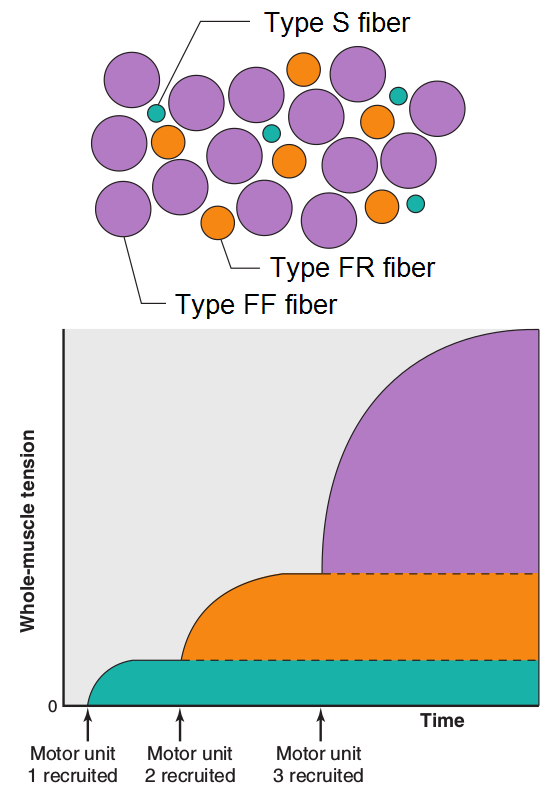
\includegraphics[width=0.5\textwidth]{Images/introduction/fiber_distribution.png}
%\caption{Figure illustrates \textbf{a)} diagram of different muscle fibers in muscle cross section, and \textbf{b)} muscle tension produced by recruitment of different types of muscle fiber. It can be noted that type S fibers are activated first and generate low force level, whereas type FF fibers are activated last and generate high forces . Adopted from Widmaier}
%\label{fig:fiber_distribution}
%\end{figure}
%
%\begin{figure}[ht]
%\centering
%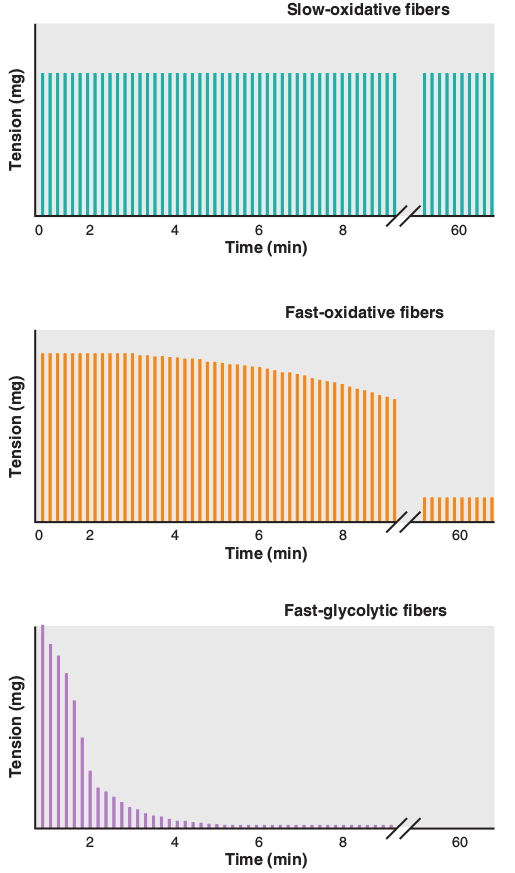
\includegraphics[width=0.5\textwidth]{Images/introduction/fiber_fatigue.png}
%\caption{Figure illustrates the time during which specific muscle fibers can remain tension. Adopted from Widmaier}
%\label{fig:fiber_fatigue}
%\end{figure}

\begin{figure*}[t!]
    \centering
    \begin{subfigure}[t]{0.45\textwidth}
        \centering
        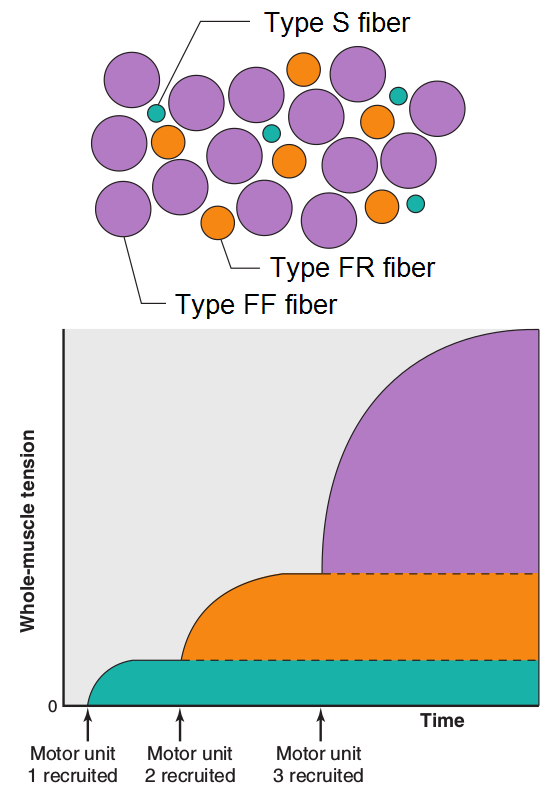
\includegraphics[height=4in]{Images/introduction/fiber_distribution.png}
        \caption{}
    \end{subfigure}%
    ~ 
    \begin{subfigure}[t]{0.45\textwidth}
        \centering
        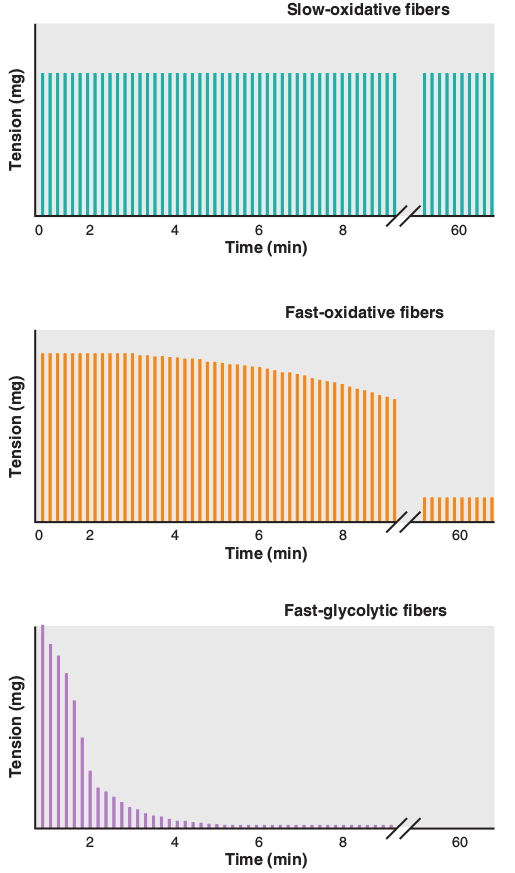
\includegraphics[height=4in]{Images/introduction/fiber_fatigue.png}
        \caption{}
    \end{subfigure}
    \caption{Figure describes characteristics of different types of muscle fibers. In \textbf{a)} is a diagram of different muscle fibers in muscle cross section (top), and muscle tension produced by recruitment of different types of muscle fiber (bottom), whereas in \textbf{b)} is the illustration of the time interval during which specific muscle fibers can remain tension. It can be noted that type I fibers are activated first, generate low force level, and are resistant to fatigue. On the other hand, type IIb fibers are activated last, generate high forces, and develop fatigue fastest. Retrieved from \citet{Widmaier2014}.}
\label{fig:fibers}
\end{figure*}


\subsection{Muscle contraction} \label{sc:contraction}

Skeletal muscles are activated voluntarily by electrochemical impulses of motor neurons. The process is described in this chapter in a summarized version. For a more detailed description, the reader is pointed to medical literature (e.g. {Widmaier2014}).

During the stable state when there are no stimuli, i.e., in the resting state, the interior of the myocyte is at a higher electrical potential than the exterior. This difference in potential is usually around 80 mV and it is caused by the higher concentration of positive ions, namely Na+, outside of the sarcolema \citep{Nazmi2016}, as shown in figure \ref{fig:depolarization}.

\begin{figure}[ht]
\centering
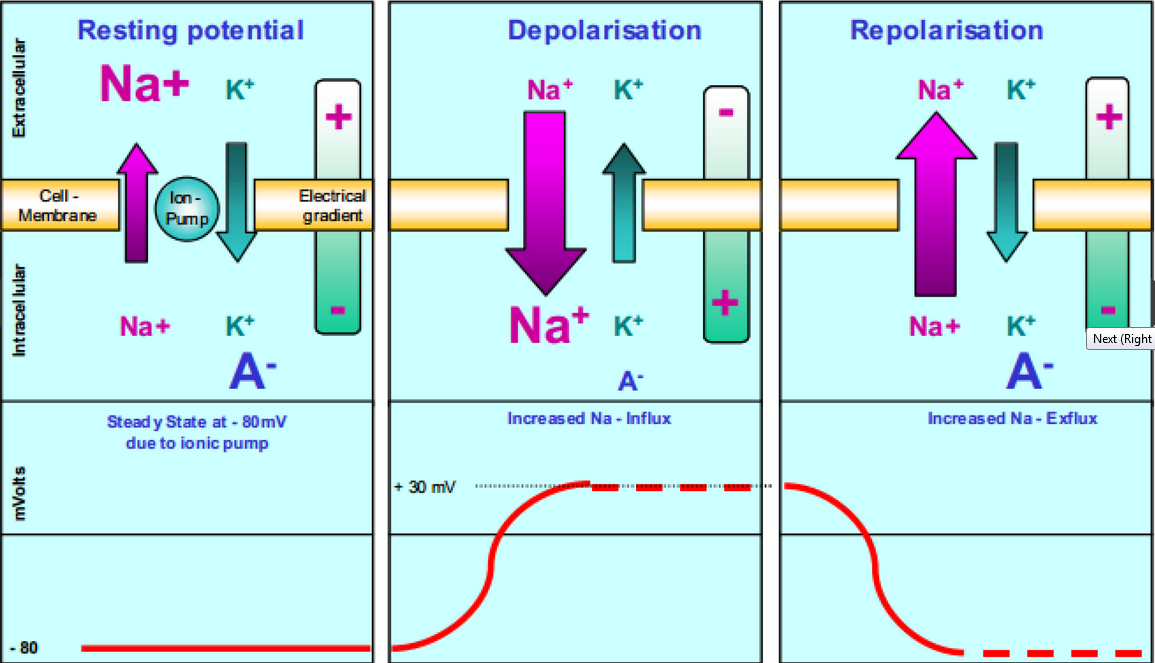
\includegraphics[width=0.95\textwidth]{Images/introduction/Depolarization.png}
\caption{Ilustration of depolarization/repolarization of the muscle fiber. Adopted from \citet{Nazmi2016}.}
\label{fig:depolarization}
\end{figure}

Motor neurons transfer nerve impulses that control the muscles from the spinal cord to the neuromuscular junction. At the nerve endings, action potentials induce the opening of calcium channels, which enables calcium from extracellular fluid to enter the axon terminals and trigger the release of the neurotransmitter \emph{acetylcholine}. Acetylcholine is released to the narrow space between the axon and the sarcolema of the myocyte, and causes the sodium channels in sarcolema to open and allow the flow of Na+ and K+ ions in both directions. Na+ ions now flow into the myoplasma by diffusion due to the higher concentration of Na+ ions outside of the membrane, but because of the similar gradient, concentrations of the K+ ions do not change a lot. This process causes depolarization of the sarcolema during which the outside potential of the muscle cell is at a lower voltage than the inside potential by around 30 mV. Depolarization is immediately followed by repolarization, a process during which the electrochemical balance and the resting potential of the cell are restored. It is achieved by flushing the Na+ ions outside of the sarcolema by the \emph{ion pump}. The process can be seen in figures \ref{fig:depolarization} and \ref{fig:action_potential_generation}.
  
\begin{figure}[ht]
\centering
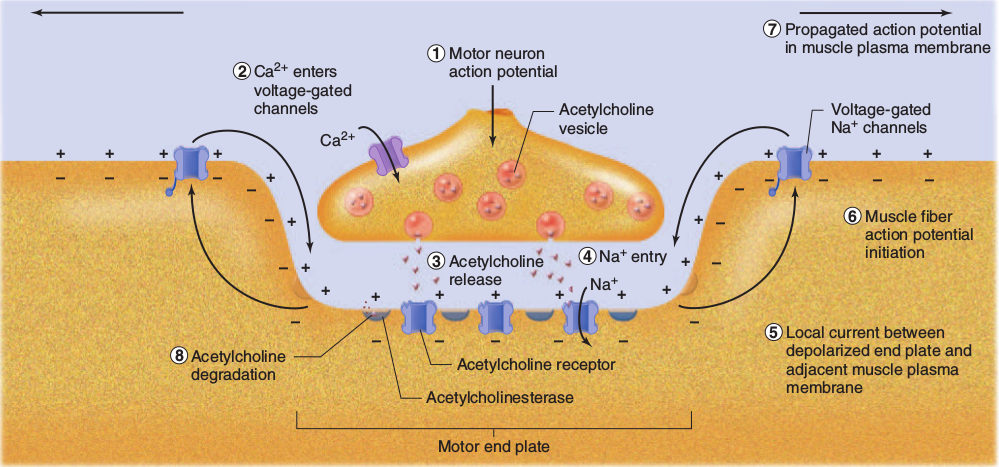
\includegraphics[width=0.95\textwidth]{Images/introduction/action_potential_generation.png}
\caption{Illustration of the generation of the muscle fiber action potential. Retrieved from \citet{Widmaier2014}.}
\label{fig:action_potential_generation}
\end{figure}
  
If the amount of acetylcoline is sufficient for the excitation, depolarization/repolarization wave, that is, action potential, propagates longitudinally from the neuromuscular junction towards the ends of the muscle fiber causing contraction \citep{Henneberg1999}. Speed of the action potential propagation is called \emph{conduction velocity} and typically ranges around 4 m/s.

Detailed analysis of muscle physiology can be found elsewhere \citep{Squire1986, Widmaier2014}.



\subsection{Muscle fatigue} \label{sc:fatigue}

According to \citet{Widmaier2014}, muscle fatigue is a decline in muscle tension as a result of a previous contractile activity. It is also characterized by a decreased relaxation rate and a lower shortening velocity of muscle fibers. Muscle fatigue is a continuous process that starts at the moment when the muscle unit activates. If a muscle keeps contracting long enough, eventually it will stop contracting because of the electrophysiological inability to maintain the contraction. This moment is called the \emph{failure point} \citep{DeLuca1984}. The failure point depends on many different physiological characteristics, but also on the number of muscle fibers and the proportion of Type I and Type II muscle fibers. Muscles with a higher proportion of Type I fibers do not fatigue easily and recover sooner than muscles composed of type II fibers. However, type II fibers are able to generate higher forces, but are also prone to fatigue \citep{Kupa1995}, as explained in section \ref{sc:contraction}.

With respect to the source of impairment, the muscle fatigue can be:

\begin{description}

\item[Peripheral fatigue] \hfill \\
	Peripheral fatigue occurs in the muscle itself, when muscle contraction is prevented because of an electrochemical imbalance. There are three main sources of peripheral fatigue:
	\begin{itemize}
		\item During sustained contraction, sarcolema of the muscle fibers become acid, and this accidifation lowers the muscle fiber conduction velocity \citep{DeLuca1984}.
		
		\item High concentration of K+ ions prevents generation of action potentials in muscle fiber \citep{Widmaier2014}. 
		
		\item Buildup of adenosine diphosphate, a byproduct of muscle contraction, slows the rate of cross-bridge cycling, affecting the relaxation, and reducing the shortening velocity \citep{Widmaier2014}.
	\end{itemize}

\item[Central fatigue] \hfill \\
	Central fatigue occurs in the central nervous system that controls the movement. It is manifested as the synchronization of neural spike trains of different motor units. This synchronization occurs because the activation of more muscle units simultaneously increases the total output force of a muscle

\end{description}

Muscle fatigue changes characteristics of the myoelectric signal. Due to the decrease of the muscle fiber conduction velocity, caused by peripheral fatigue, and due to the synchronization of the firing times caused by central fatigue, there is a shift of energy in the frequency spectrum of the myoelectric signal towards lower frequency, as shown in figure \ref{fig:fatigue} \citep{DeLuca1984}. Another indicator of muscle fatigue is the increase of amplitude of the surface electromyographic signal. This increase occurs due to two main reasons:
\begin{itemize}
\item The tissue between muscle fibers and the recording electrodes positioned on the surface of the skin (e.g. fat layers, skin, etc.) has low-pass filtering properties. The propagating electrical wave caused by the action potential is low pass filtered before it is recorded by the electrodes mounted on the surface of the skin. Since the power of the propagating wave shifts towards lower frequencies because of the fatigue, the amplitude of the recorded signal increases.

\item Due to the synchronization of firing patterns caused by the central fatigue, the amplitude of the recorded signal increases. 
\end{itemize} 

\begin{figure}[ht]
\centering
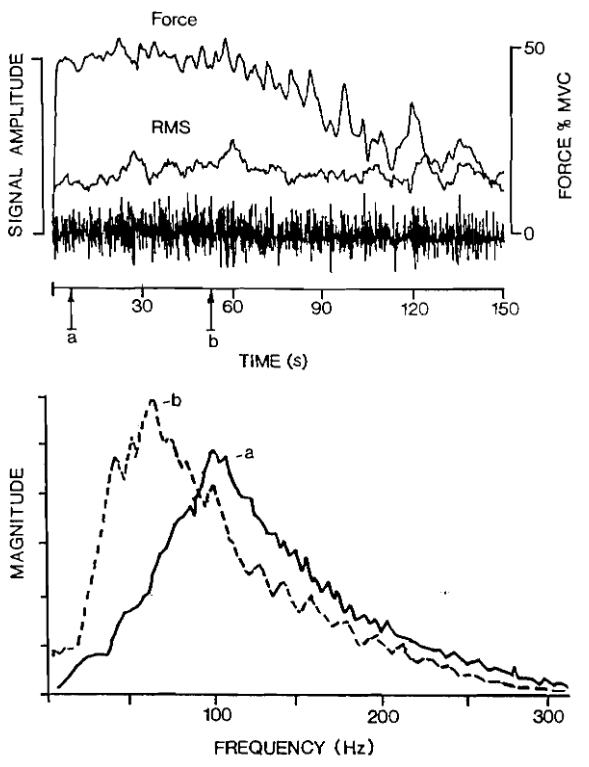
\includegraphics[width=0.45\textwidth]{Images/introduction/fatigue.png}
\caption{Illustration of the force and the myoelectric signal recorded on the surface of the skin during fatiguing exercise (top), and the frequency spectra of the corresponding signal (bottom) recorded at the beginning of the exercise (a), and at the time when the force started decreasing (b). Retrieved from \citet{DeLuca1984}.}
\label{fig:fatigue}
\end{figure}

There are many studies exploiting these changes in the myoelectric signal to estimate and monitor muscle fatigue. Most of the approaches are based on monitoring frequency characteristics of the signal. One of the simplest measures is the number of zero-crossings \citep{Hagg1981}, but because it is very sensitive to noise, it is rarely used. Mean and median frequencies are often used in literature \citep{Lindstrom1977, Merletti1997, Stulen1981}, as are more advanced time-frequency processing methods \citep{Knaflitz1999, Cifrek2000, Georgakis2003, Srhoj-Egekher2011a}.


\section{Surface electromyography}

The muscle unit action potential (MUAP) is a combination of action potentials generated by all muscle fibers belonging to that motor unit, whereas the electromyographic signal (EMG) is a superposition of electrical activity (propagating action potentials) produced by all muscle units. 

\subsection{Intramuscular vs. surface electrmyography}

There are two main types of electromyographic measurements: 
\begin{description}
\item[Surface EMG (sEMG)] This is a non-invasive type of EMG measurement where electrodes are positioned on the surface of the skin. Two types of electrodes are used: wet electrodes, which are used in combination with a conductive gel that provides high signal quality, and dry electrodes, which can be applied directly to the skin. Although wet electrodes are mostly used, the signal quality deteriorates during recording because of drying of the gel. Since this effect is not present with dry electrodes, some authors recommend using this type of electrodes for long-term recordings \citep{Merletti2009, Hakonen2015}.

\item[Intramuscular EMG (iEMG)] This is an invasive type of recording which implies insertion of a needle or a wire electrode under the skin \citep{Marateb1999}. This type of recording is used for a precise measurement of a narrow volume, for example couple of muscle fibers. It has a high signal-to-noise ratio, but causes discomfort in subjects. It is often used in clinical practice because it can detect abnormal functionalities. For example, action potentials of spontaneously contracting single muscle fibers can be measured. These potentials are an important sign of deinnervation, but cannot be recorded using sEMG \citep{Merletti-book}.
\end{description}

Although iEMG signal usually has higher quality (in terms of signal-to-noise ratio), it was shown that similar results in the identification of upper-arm motor tasks can be obtained using both approaches \citep{Hargrove2007}. Since sEMG is non-invasive, it is usually the preferred method in myocontrol and has become a gold standard of the upper-limb prosthetics \citep{Kamavuako2013}. Moreover, although the narrow volume scope of iEMG can often be beneficial, especially in clinical applications regarding activation of a single muscle unit, it does not provide information on other parts of the muscle. For that reason, sEMG can be more appropriate because it simultaneously records action potentials of a large muscle area. Depending on the application, that can also be a serious drawback because if there are several active muscles in a small volume, myoelectric activity of both muscles will be recorded, i.e., there will be \emph{crosstalk} between muscles. 


\subsection{Origin of surface electromyographic signal}
The surface electromyographic signal is the sum of the electrical activity of muscle units recorded on the surface of the skin. From the statistical point of view, the EMG signal can be considered as a non-stationary stochastic process whose probability density function is a Gaussian function. \citep{DeLuca1984, DeLuca1979}. Since muscle fibers are activated by the impulse train of the innervating motor neurons, i.e. neural drive to the muscle, sEMG is the convolution of the motor neuron spike trains by the motor unit action potential recorded on the electrodes \citep{Farina2010, Farina2014}:
%Surface EMG usually has frequency bandwidth up to 300 Hz and amplitude up to couple of milivolts \citep{Merletti-book}.

\begin{equation}
sEMG(t) = \sum_{i=1}^{M} \sum_{j=-\infty}^{+\infty} MUAP_i(t)\,\, \delta(t-t_{i,j})
\end{equation}

, where $M$ is the number of active motor units, $MUAP_i(t)$ is the action potential waveform of the $i^{th}$ motor unit recorded by the electrodes, and $t_{i,j}$ is the time of the discharge of the $i^{th}$ motor neuron. This model assumes there is no interference and that the neuromuscular junction never fails, which is not the case. In the equation, $MUAP_i(t)$ is related to the electrophysiological state of the muscle fiber membranes and the conduction properties of the tissue through which the potential propagates, whereas neural information is contained in motor neuron spike trains $\delta(t-t_{i,j})$ \citep{Farina2014b}. With respect to the muscle fatigue explained in the previous section (section \ref{sc:fatigue}), peripheral fatigue affects $MUAP_i(t)$, whereas central fatigue has an effect on $\delta(t-t_{i,j})$ term. It is important to notice that following this model, sEMG reflects all motor control information that is present in the motor neurons. For that reason, it is more appropriate to extract motor control information carried by motor neurons using sEMG, than directly by invasive measurement of the electrical potential of the motor neuron. The advantage of the sEMG is that multiple fibers are activated simultanously, generating a bioelectrical signal with a relatively high SNR, which can be measured on the surface of the skin. In this context, sEMG can be considered as the amplified neural signal, whereas the muscle can be considered as a biological amplifier of nerve activity \citep{Farina2014}. Origin of the sEMG signal can be seen in figure \ref{fig:EMG_origin}.
\begin{figure}[ht]
\centering
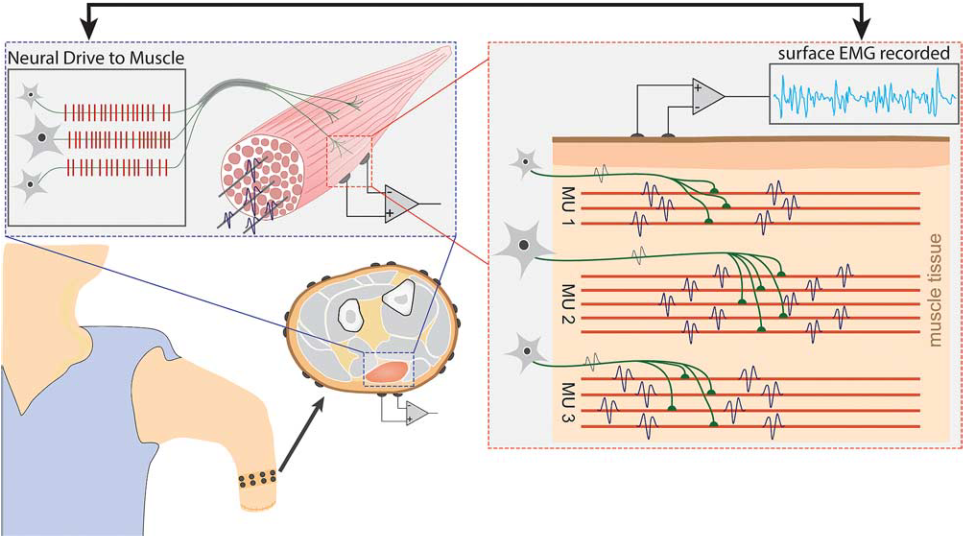
\includegraphics[width=0.90\textwidth]{Images/introduction/EMG_origin.png}
\caption{The sEMG signal is a superposition of motor unit action potentials recorded on the electrodes convoluted by the belonging motor neuron spike train. Retrieved from \citet{Farina2014}.}
\label{fig:EMG_origin}
\end{figure}

Described in the frequency domain, the motor unit action potential spike train also provides the neural and the peripheral information:

\begin{equation}
P_{sEMG}(f) = \sum_{i=1}^{M} P_{ST_i}(f) \, \, \big\vert \Phi_{MUAP_i}(f) \big\vert^2
\end{equation}

,where $P_{sEMG}(f)$ is the power spectrum of the sEMG signal, $\Phi_{MUAP_i}(f)$ is the Fourier transform of the $MUAP_i$, and $P_{ST_i}(f)$ is the power spectrum of the neural spike train that innervates it, where it is assumed that spike trains are uncorrelated processes \citep{Farina2014}.

In case of a constant average discharge rate of spike trains, assuming that it is a stationary process, the spike train power spectrum can be calculated as \citep{Farina2014}:

\begin{equation}
P_{ST_i}(f) = DR_i \left[ 1- \big\vert Q_i(f)\big\vert^2 \right] + DR_i^2  \big\vert Q_i(f)\big\vert^2 \,  \sum_{n=-\infty}^{+\infty} \delta(f - n DR_i)
\end{equation}

, where $DR_i$ is the average discharge rate, and $Q_i(f)$ is the Fourier transform of the probability density function of the inter-spike interval variability. The first term in the equation is dominant and equal to $DR_i$ for frequencies greater than 10 - 20 Hz, as proven previously \citep{Lago1977, Farina2014}. Therefore, the power spectrum of the sEMG signal can be estimated as:

\begin{equation}
P_{sEMG}(f) \approx  \sum_{i=1}^{M} DR_i \, \big\vert \Phi_{MUAP_i}(f) \big\vert^2
\end{equation}

Power of the sEMG signal $P$ can be obtained in the frequency domain as:

\begin{equation}
P = \int_0^{+\infty} P_{sEMG}(f)  \, df  \, \approx \, \sum_{i=1}^{M} DR_i \, \int_0^{+\infty} \big\vert \Phi_{MUAP_i}(f) \big\vert^2 \, \approx \, \sum_{i=1}^{M} DR_i \,E_i
\end{equation}

,where $E_i$ is the energy of $MUAP_i$. It can be noted that the power of the sEMG is the sum of energies of action potentials of motor units weighted by their discharge rate. When the force of a contraction is increased, the power of the sEMG increases also because of the activation of additional motor units ($M$ increases) and because of the increase of the the average discharge rate of motor neuron action potentials ($DR_i$ increases). On the other hand, when the muscle is fatigued, the conduction velocity of muscle fibers decreases and the power spectrum of the muscle fiber action potentials shifts towards lower frequencies, as explained in section \ref{sc:fatigue}. Due to this effect, energy of MUAPs recorded on the electrodes can increase, leading to an increase of sEMG power ($E_i$ increases).

Given the fact that there is a large variability between shape, and amplitude of MUAP with respect to the electrode position and the tissue conduction characteristics, the association between the power of the sEMG and the neural drive can also have a very high variability, depending on the individual subject and the muscle \citep{Farina2014}. 

\subsection{Recording electrodes}
Depending on the number of electrodes used for the recording, the following classification exists: single-channel recording in a monopolar mode, single channel recording in a bipolar mode (differential recording), recording using a linear electrode array, and high-density EMG, as shown in figure \ref{fig:electrode_types}.
\begin{figure}[ht]
\centering
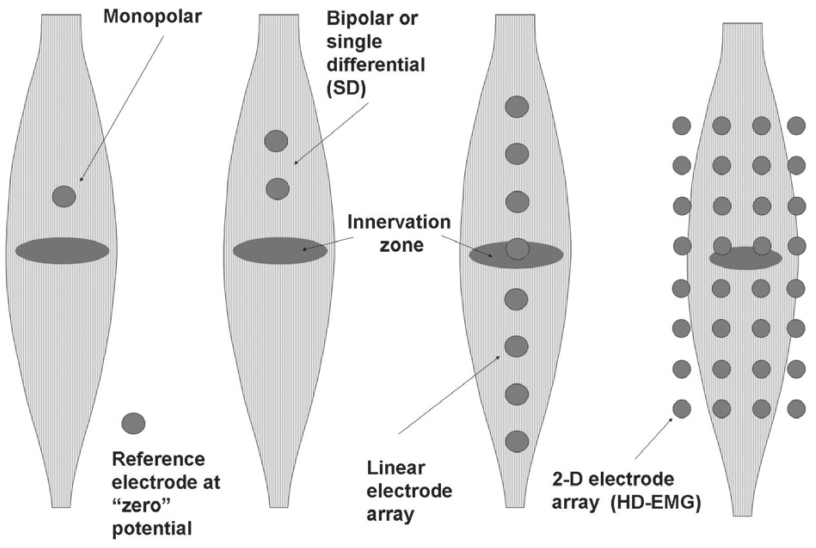
\includegraphics[width=0.70\textwidth]{Images/introduction/electrode_types.png}
\caption{Four types of recording surface EMG signal: monopolar, bipolar, linear electrode array, HD-EMG. Figure was modified from \citet{Merletti2010}.}
\label{fig:electrode_types}
\end{figure}

In the single-channel monopolar recording, a single electrode is positioned over the muscle, whereas the reference electrode is positioned over the place that does not generate electrical activity. On the other hand, the single-channel bipolar electrode configuration is often used, in which a signal is the difference of potential between the two electrodes. This configuration is traditionally preferred because of the lower interference and a higher signal-to-noise ratio \citep{Merletti-book}. General recommendation is that the inter-electrode distance is around 20 cm \citep{Hermens1999}, but the optimal distance depends on many factors, as briefly explained in \citep{Hakonen2015}. For both monopolar and bipolar single channel recordings it is recommended that the electrodes are positioned between the innervation zone and the tendon. Exact recommendations can be found in the findings of the SENIAM project \citep{Hermens1999}.

The linear electrode array consists of multiple electrodes positioned at an equal distance along the line of muscle fibers, following the direction of the propagation of the action potentials. Measurements recorded using this type of electrodes provide more information on the muscle than a single channel recording. For example, it can be used for the estimation of the conduction velocity, as shown is figure \ref{fig:conduction_velocity} \citep{Merletti-book}.
\begin{figure}[ht]
\centering
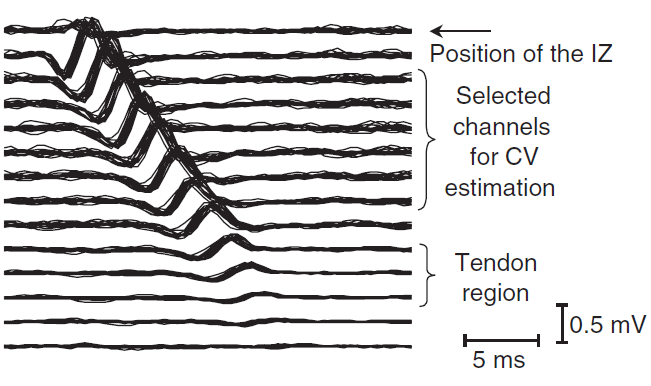
\includegraphics[width=0.60\textwidth]{Images/introduction/conduction_velocity.png}
\caption{Estimating the location of the innervation zone (IZ) and the conduction velocity (CV) using averaged MUAPs recorded using linear electrode array. Figure was retrieved from \citet{Merletti-book}.}
\label{fig:conduction_velocity}
\end{figure}

Technological advancement of the EMG acquisition systems enables the use of high-density electromyography (HD-EMG) \citep{Zwarts2004}. Using an array of closely spaced electrodes organized in a quadrature grid, multiple EMG channels are recorded over the wide area of the muscle. The electrodes used for the HD-EMG recording can be seen in figure \ref{fig:electrode}. This type of a recording is more reliable because it can record activations in different parts of the muscle and increase redundancy. HD-EMG is the only EMG recording approach that allows insights into the spatial distribution of motor units in a muscle. By observing the amplitude or the intensity of signals recorded in different channels, it is possible to analyze how different muscle regions activate depending on the joint position \citep{Vieira2010}, the contraction level \citep{Holtermann2005}, and the duration of movement and fatigue \citep{Tucker2009, Staudenmann2014}. Moreover, since muscles do not activate homogeneously, sEMG recorded using a single channel has some serious drawbacks, which can be overcome by using 2D electrode arrays. For example, Zwartz and Stegeman pointed out that the single channel EMG disregards important spatial aspects of MUAP propagation, which are essential for the force-generating capacity of the muscle, and, if not well addressed, can lead to incorrect conclusions \citep{Zwarts2003}. 
\begin{figure}[ht]
\centering
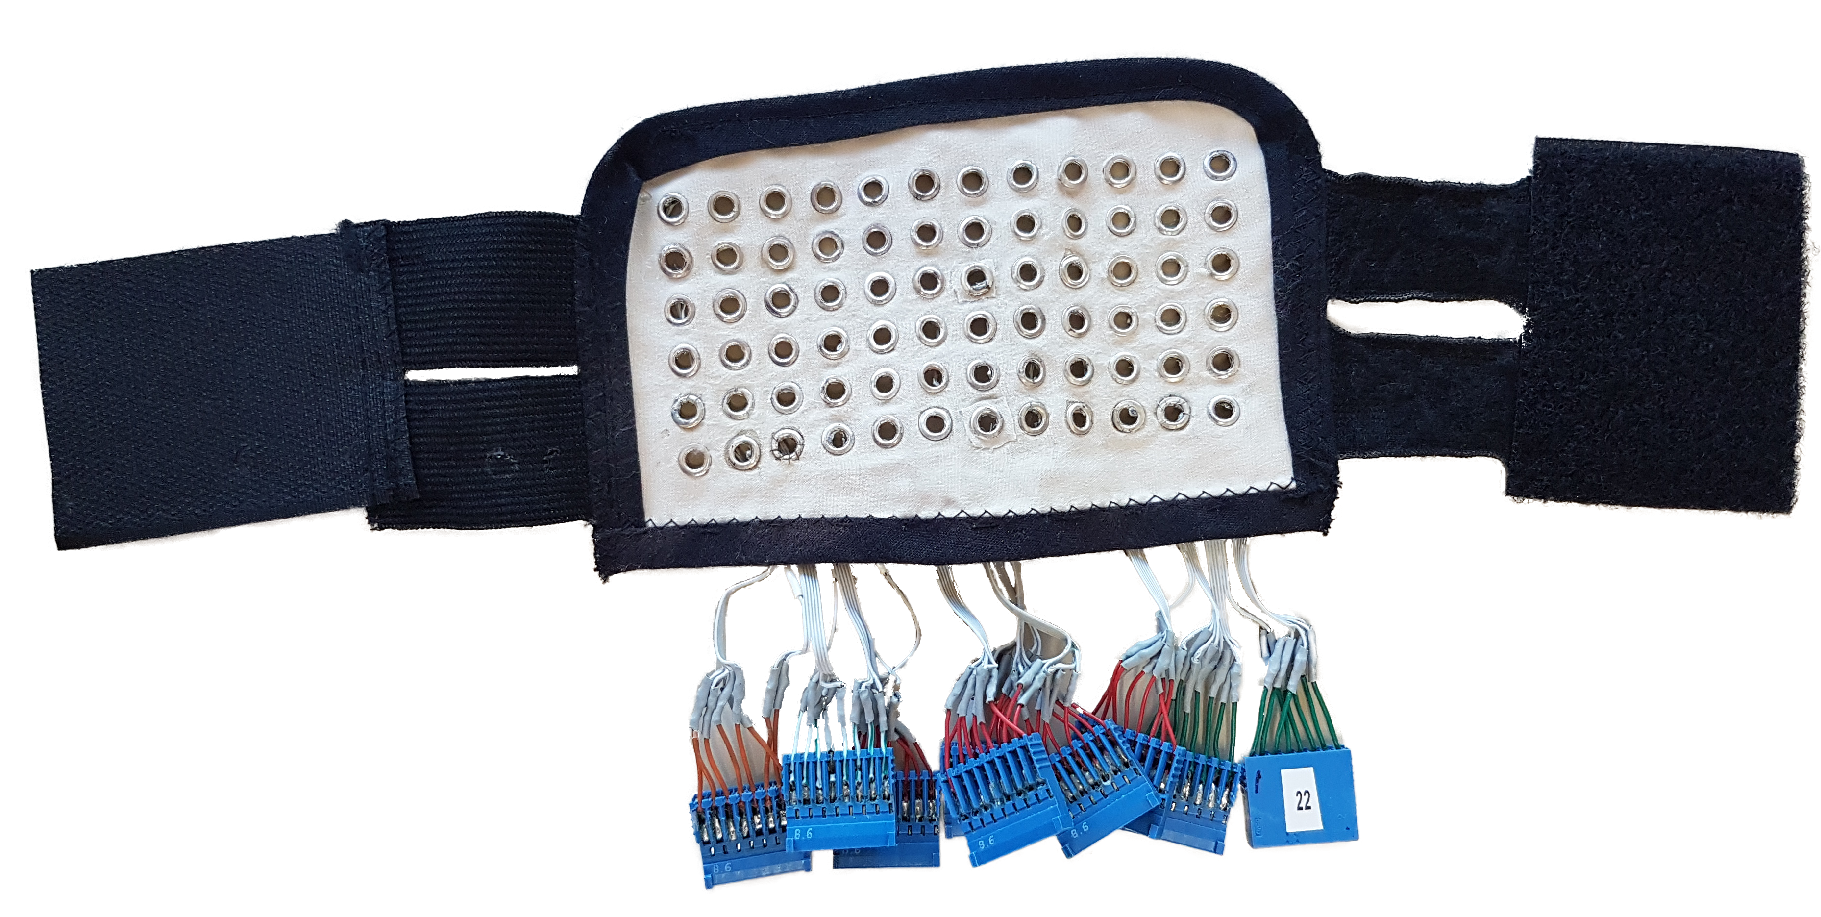
\includegraphics[width=0.7\textwidth]{Images/introduction/electrode2.png}
\caption{The figure represents HD-EMG electrode that was used for recording of the database used in this thesis.}
\label{fig:electrode}
\end{figure}

In addition, the activation of individual motor units, i.e. individual motor neuron spike train, can be extracted from the HD-EMG recordings using blind source separation methods \citep{Holobar2007, Holobar2010}, which can be a valuable information in the force estimation because the motor unit recruitment and the firing frequency depend primarily on the force level \citep{Merletti-book}. Several authors have used this approach instead of the traditional one based on the intramuscular (invasive) EMG. One of the obvious advantages of this method is that it is safe and not painful. Using this technique, Holobar et al. were able to extract 6 to 7 motor units starting from contractions at 5\% of maximal voluntary contraction (MVC) and up to 20\% MVC with associated discharge rates between 10 pps and 12 pps \citep{Holobar2010}. However, one of the current limitations is that it can only be performed during isometric contractions and the intensity of isometric contraction must remain constant during the measurement.

HD-EMG recordings also allow calculation of two-dimensional activation maps where intensity of each pixel represents the intensity of a corresponding EMG channel (see figure \ref{fig:HD-EMG}). Consequently, the information on spatial distribution of the EMG intensity over the muscle is provided. Recent studies show that changes in the spatial activation pattern are related to the duration of movement and fatigue \citep{Tucker2009, Staudenmann2014}, the position of joint \citep{Vieira2010} and the level of contraction \citep{Holtermann2005}. Furthermore, these HD-EMG activation maps can also be used to determine multiple innervation zones \citep{Marateb2016}.
\begin{figure}[ht]
\centering
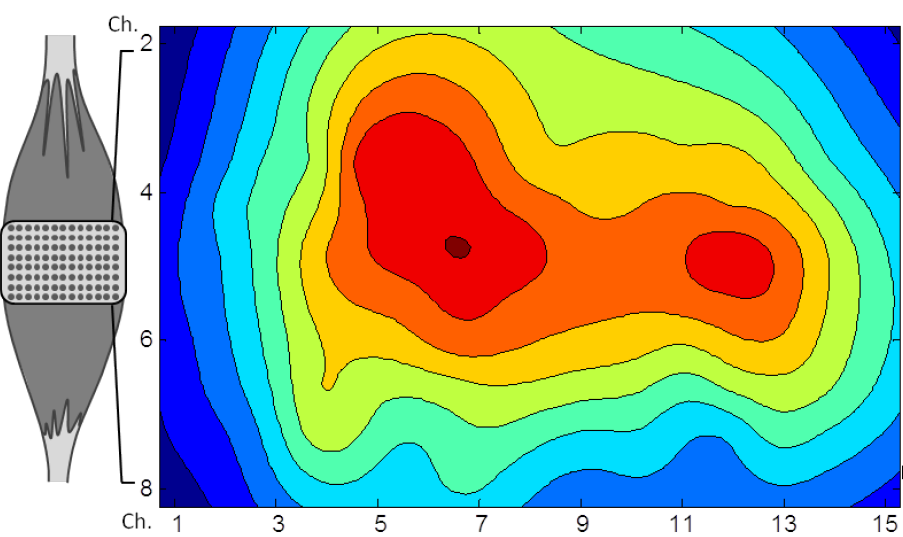
\includegraphics[width=0.95\textwidth]{Images/introduction/HD-EMG.png}
\caption{The figure represents the HD-EMG activation map recorded on the biceps brachii muscle during flexion. Distinct activation of the two heads can be noticed in the map. Modified from \citet{Monica-thesis}.}
\label{fig:HD-EMG}
\end{figure}

Moreover, these HD-EMG activation maps also proved to be valuable in the task identification using pattern recognition. Spatial characteristics of HD-EMG change depending on the  task, but also depending on the force the subject is applying, and form repeatable muscle activation patterns that can be used in the identification of the motion intention \citep{Rojas-Martinez2012}.

However, HD-EMG can be corrupted by low quality channels, which are a common issue in measurements due to well-known artifacts, such as: electrode displacement, bad electrical contact between skin and the electrode, movement of cables, electromagnetic interference, etc. \citep{Clancy2002b}. Affected channels differentiate themselves in amplitude and spectral content. To cope with this problem, Rojas-Martínez et al. developed an expert system for detection, removal and interpolation of HD-EMG channels corrupted by artifacts \citep{Rojas-Martinez2012}. On the other hand, Ghaderi and Marateb used image inpainting and surface reconstruction methods to reconstruct the corrupted activation map \citep{Ghaderi2017}.


\section{Task identification using pattern recognition}

Given the one to one relationship between the neural commands and the activation of motor units in the muscles, surface electromyography (sEMG) has been used for more than a half of century as a noninvasive and natural way of extracting motor control information for identification of motion intention. Such information can be used in numerous applications in rehabilitation engineering, e.g., prosthetics \citep{Li2010, Young2013, Stango2015}, exoskeletons \citep{VacaBenitez2013} and rehabilitation robots \citep{Dipietro2005, Marchal-Crespo2009, Cesqui2013}.

Ideally, a system for the identification of motion intention should fulfill the following criteria \citep{Farina2014}:
\begin{itemize}
\item should provide simultaneous activation of multiple degrees of freedom
\item should provide proportional control
\item should be insensitive to changes in electrode - skin impedance,
\item should be adaptive to changes during the use, i.e. fatigue, electrode-skin impedance change due to sweating and drying of conductive gel
\item should be insensitive to precise position of electrodes
\item should have fast and easy training procedure (ideally none)
\item should provide real time identification, i.e. time delay less than 300 ms \citep{Oskoei2007}
\item should have low computation complexity which enables implementation in a battery-powered device
\end{itemize}

In most of the commercial prosthesis \citep{Parker1986}, sEMG of two muscles is recorded. In this simple scheme a single Degree-of-Freedom (DoF) can be controlled: the EMG amplitude of one muscle controls the output of one direction, whereas the EMG amplitude of the other muscle controls the other direction. If a prosthesis needs to operate in multiple DoFs, a subject needs to switch between active DoFs either by co-contraction, or by pressing a switch button. In any case, the method is not intuitive nor efficient for the user \citep{Farina2014}.

Pattern recognition is an alternative to conventional control algorithms and has been extensively used in research institutions during the last decades \citep{Hakonen2015, Farina2014, Nazmi2016}. The prerequisite of using pattern recognition for task identification is the presence of a pattern that can be extracted from the EMG signal. Major advancement over conventional switching myocontrol is the possibility of instant selection of any of the predefined movements.

However, although pattern recognition improves the possibilities of extraction of motion intention, it has several serious limitations. Therefore, there is still a large gap between use of pattern recognition in research and in practice in rehabilitation institutes and in users' homes \citep{Jiang2012}. The pattern recognition approach does not support proportional and simultaneous control for multiple motor tasks. Any task that requires more than one DoF must be performed sequentially. This type of control prevents the user from achieving a fluid movement, but also demands planning of movement execution. However, several authors recently proposed solutions which enable simultaneous control \citep{Young2013, Kamavuako2013, Baker2010}. For example, Young et al. propose a system of parallel classifiers that use conditional probabilities to separate between combination of tasks \citep{Young2013}. On the other hand, there are also publications proposing solutions for the proportional control. Fougner et al. prepared a review on the topic \citep{Fougner2012}. The main idea behind this approach is that the muscle force can be estimated using the EMG signal \citep{Staudenmann2010}. 

On the other hand, one of the disadvantages of pattern recognition is the fact that in spite of the high accuracy, an error could lead to a completely unwanted task. Furthermore, although the identification rate is usually very high during the stationary task, errors often occur during transition between tasks. These problems can be partially prevented by, for example, employing the majority voting principle \citep{Englehart2003}, or the decision-based velocity ramp that attenuates the velocity of a movement after the change of a task \citep{Simon2011}. % Englehart 300 ms

Although crosstalk is usually considered as a negative interference in electromyography, if it is consistent and repeatable, some authors argue that it can provide a discriminative power in task identification \citep{Farina2014}. However, for some approaches it has a negative influence \citep{He2015}. To resolve this issue, source separation methods can be used to separate EMG activity of adjacent muscles \citep{Farina2004, Holobar2014}. This can be a powerful tool in task identification \citep{Naik2007}, because it could separate contributions of individual muscles in the myoelectric signal, and, therefore, minimize crosstalk effect from nearby muscles. Consequently, extracted features would characterize only the target muscles.


According to Oskoei et al. pattern-recognition-based task identification approach includes four main modules \citep{Oskoei2007}:
\begin{description}
\item[Data segmentation:] \hfill \\
Comprises various techniques and methods that are used to handle data before feature extraction. Recording must be divided in time segments on which identification will be performed. Selection of duration of time segment has an effect on the identification. Features calculated on wider segments usually have lower variability, and, consequently, higher repeatability and a stronger pattern, which increases the identification rate. On the other hand, the output of the classifier should be as fast as possible in order to be used in real time.  Therefore, the shorter the window, the shorter the response time will be. General recommendation is that the total delay of the system should be less than 300 ms \citep{Oskoei2007, Englehart2003}. 

\item[Feature extraction:] \hfill \\
This module computes preselected features for classification. Selection and extraction of features is one of the most critical stages in myoelectric control design and there are many features suggested in the literature. 

\item[Classification:] \hfill \\
A classification module recognizes signal patterns, and classifies them into predefined categories. Due to the complexity of biological signals, and the influence of physiological and physical conditions, the classifier should be adequately robust.

\item[Controller:] \hfill \\Generates output commands based on the output of the classifier and control schemes. Post-processing methods are often included in this module. For example, majority voting is often applied after classification to eliminate destructive jumps and to make a smooth output.
\end{description}

Many studies agree that the selection of the pattern recognition technique does not have a big influence on the task identification \citep{Hakonen2015}. Therefore, simple and fast classifiers are preferred. Linear discriminant analysis has become the 'gold standard' in the field of myoelectric control because of these properties \citep{Tkach2010, Li2014, Hakonen2015}. Although this classifier assumes multivariate normal distribution of classes, experiments proved that it performs well even if the normality assumption has not been met \citep{Grouven1996}.

Features, on the other hand, have a major influence on the identification results \citep{Englehart1999, Tkach2010}. Therefore, there are many features proposed in the literature focused on improving the rate of identification of motion intention:

\begin{description}
\item[Time domain features:] \hfill \\
Mean absolute value \citep{Hudgins1993}, integrated EMG \citep{Park1998}, variance \citep{Park1998, Zardoshti1995}, root mean square \citep{Farrell2008}, waveform length \citep{Hudgins1993}, zero crossing \citep{Hudgins1993}, log detector \citep{Tkach2010}, Wilson amplitude \citep{Zardoshti1995}, slope sign change \citep{Hudgins1993}, autoregressive coefficients \citep{Hargrove2007}, cepstral coefficients \citep{Park1998}, mean absolute value slope \citep{Phinyomark2012}, histogram of EMG \citep{Phinyomark2012, Zardoshti1995}
\item[Frequency domain features:] \hfill \\
Mean frequency \citep{Phinyomark2012b}, median frequency \citep{Phinyomark2012b}, modified mean frequency \citep{Phinyomark2009}
\item[Time-frequency domain features:] \hfill \\
Short time Fourier transform \citep{Englehart2003b, Englehart2001}, continuous wavelet transform \citep{Englehart2003b, Englehart2001}, discrete wavelet transform \citep{Englehart2003b}, stationary wavelet transform \citep{Englehart2003b}, wavelet packet transform \citep{Englehart2003b, Englehart2001, Chu2006}
\item[Spatial domain features:] \hfill \\
Experimental variogram \citep{Stango2015}, center of gravity \citep{Rojas-Martinez2012, Rojas-Martinez2013}
\end{description}

Time domain features are commonly used because they achieve high identification accuracy and are computationally efficient \citep{Hakonen2015}.

Since spatial distribution contains a lot of information on the muscle, features derived from this information are acknowledged as valuable in the identification of motion intention \citep{Stango2015, Hakonen2015, Rojas-Martinez2013}. For example, Stango et al. \citep{Stango2015} used spatial characteristics of HD-EMG recording of the forearm muscles to identify 8 hand and wrist tasks (4 degrees of freedom). They fed the support vector machine classifier with a statistical measure of spatial correlation, i.e. variogram and achieved high identification results (95\% accuracy). Furthermore, they proved that proposed spatial features are robust to the electrode shift.

Most of the pattern recognition identification methods are subject-specific. They usually achieve very high identification results, but require a time consuming training procedure for every patient individually. This could be avoided by building a single identifier for a group of patients, i.e. a group-specific identifier. However, inter-subject variability is a big concern in the design of a group-specific pattern recognition-based identifier. Individuals differ from each other in a lot of physiological parameters, e.g., conductivity of subcuntaneous tissue, and limb dimension. Nevertheless, by comparing HD-EMG activation maps between normal subjects it has been shown that inter-subject activation patterns exist for different tasks and levels of contraction \citep{Rojas-Martinez2012}.

Rojas-Martínez et al. demonstrated that by using intensity and spatial features extracted from activation maps it is possible to construct an inter-subject identification method based on the LDA classifier not only for different tasks, but also for different effort. Authors reported that in healthy subjects identification performance improves by adding spatial features in the identification, which proves that spatial distribution is less sensitive to inter-subject variability. They achieved a sensitivity higher than 75\% for identification of four upper-limb tasks at three different effort levels and more than 90\% sensitivity when identifying only four tasks, regardless of the effort level. Also, they reported higher classification results when using classification in two steps (in the first step the task is classified, and in the second step the level of effort), rather than a single step classification.


\section{Application to patients with neuromuscular impairment}

%\begin{figure}[ht]
%\centering
%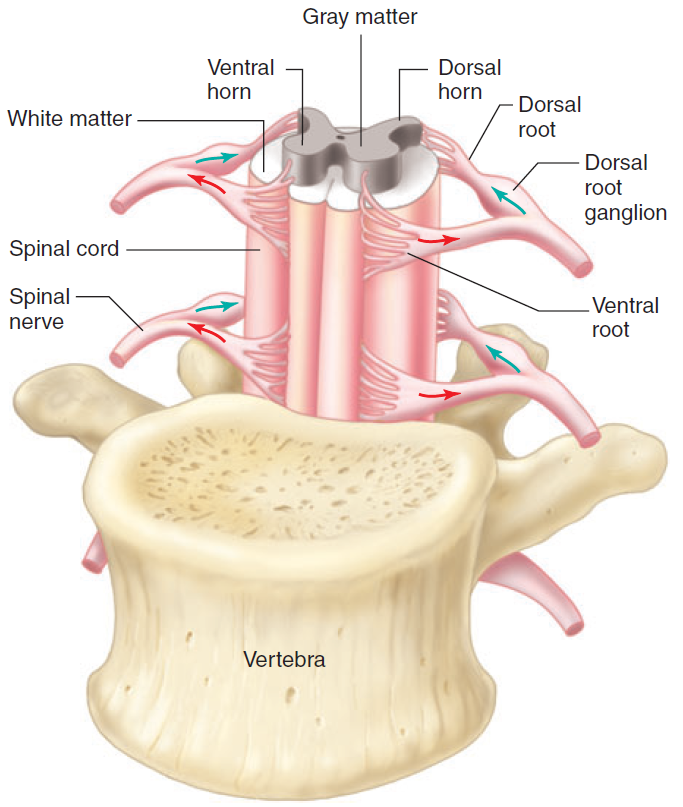
\includegraphics[width=0.50\textwidth]{Images/introduction/vertebra.png}
%\caption{Ventral view of the section of the spinal cord. The direction of transmission of neural activity is noted by arrows. Retrieved from \citet{Widmaier2014}.}
%\label{fig:vertebra}
%\end{figure}
%
%\begin{figure}[ht]
%\centering
%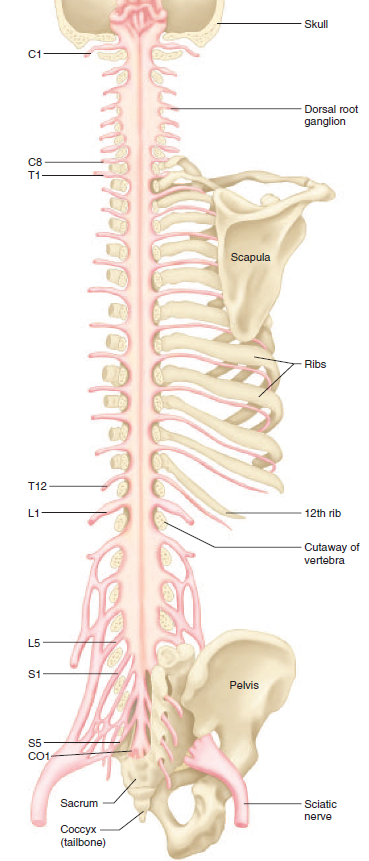
\includegraphics[width=0.50\textwidth]{Images/introduction/spinal_cord.png}
%\caption{Dorsal view of the spinal cord. Parts of the skull and vertebrae have been cut away. In general, the eight cervical nerves (C) control the muscles and glands and receive sensory input from the neck, shoulder, arm, and hand. The 12 thoracic nerves (T) are associated with the chest and abdominal walls. The five lumbar nerves (L) are associated with the hip and leg, and the five sacral nerves (S) are associated with the genitals and lower digestive tract. Retrieved from \citet{Widmaier2014}.}
%\label{fig:spinal_cord}
%\end{figure}
%
%
%\begin{figure}[ht]
%\centering
%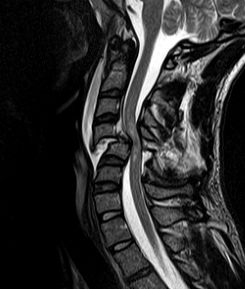
\includegraphics[width=0.50\textwidth]{Images/introduction/SCI.png}
%\caption{Magnetic resonance imaging scan of cervical spine of patient with SCI. There is a fracture and dislocation at C4 vertebra, compressing spinal cord. Figure was retrieved from \citet{Korolev2012}.}
%\label{fig:SCI}
%\end{figure}
Physical injury to the brain, spinal cord, or nerves, is usually the cause of neurological disorders. According to World Health Organization, each year there are 500 000 spinal cord injuries and 15 million strokes (of which 5 million result with death and 5 million with permanent disability) every year. Furthermore, the number of people who are older than 60 years will increase to 22\% of the world population by 2050 and will count 2 billion people. Unfortunately, in affected patients motor control can be impaired as a result of damaged nerves and they often suffer from uncoordinated movements, lack of force, and spasticity. Common manifestations of upper extremity motor impairment include muscle weakness, impaired motor control, and changes in muscle tone. These impairments induce disabilities in common daily life tasks like reaching and holding objects. During the recovery process, rehabilitation robots that stimulate neuroplasticity are commonly used \citep{VacaBenitez2013, Dipietro2005, Marchal-Crespo2009, Cesqui2013}. 

Spinal cord is a slender cylinder of soft tissue, lying protected within the vertebral column \citep{Widmaier2014}. In the center is gray matter, the butterfly-shaped cross section area composed of interneurons, the cell bodies and dendrites of efferent and afferent neurons, the entering fibers of afferent neurons, and glial cells. It is surrounded by white matter, consisted of groups of myelinated axons. At each vertebra and at each side of the spinal cord, efferent nerves leave the cord at ventral side, whereas afferent nerves enter the spine at the dorsal side (see figure \ref{fig:spinal_cord}b). A short distance from the cord, the dorsal and ventral roots from the same level combine to form a spinal nerve, which innervates a specific part of the body and carries motor control information to muscles. In general, the eight cervical nerves (C) control the muscles and glands and receive sensory input from the neck, shoulder, arm, and hand (see figure \ref{fig:spinal_cord}a). The 12 thoracic nerves (T) are associated with the chest and abdominal walls. The five lumbar nerves (L) are associated with the hip and leg, and the five sacral nerves (S) are associated with the genitals and lower digestive tract.

\begin{figure}
\centering

\tabskip=0pt
\valign{#\cr
  \hbox{%
    \begin{subfigure}[b]{.48\textwidth}
    \centering
    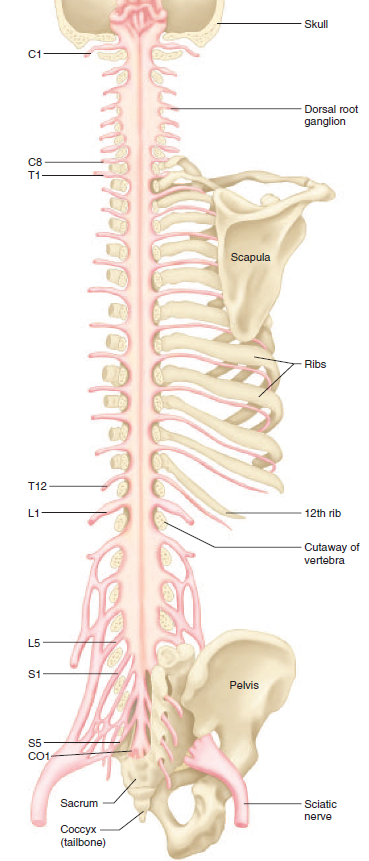
\includegraphics[width=\textwidth]{Images/introduction/spinal_cord.png}
    \caption{Retrieved from \citet{Widmaier2014}.}
    \end{subfigure}%
  }\cr
  \noalign{\hfill}
  \hbox{%
    \begin{subfigure}{.48\textwidth}
    \centering
    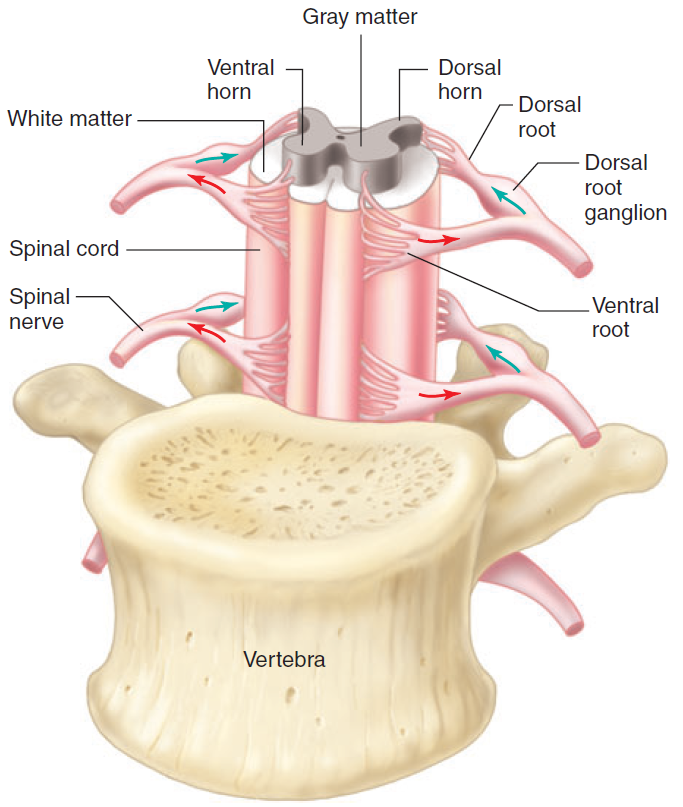
\includegraphics[width=\textwidth]{Images/introduction/vertebra.png}
    \caption{Retrieved from \citet{Widmaier2014}.}
    \end{subfigure}%
  }\vfill
  \hbox{%
    \begin{subfigure}{.43\textwidth}
    \centering
    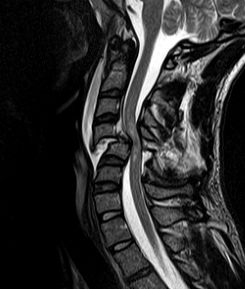
\includegraphics[width=\textwidth]{Images/introduction/SCI.png}
    \caption{Retrieved from \citet{Korolev2012}.}
    \end{subfigure}%
  }\cr
}
\caption{Figure shows \textbf{a)} dorsal view of the spinal cord. Parts of the skull and vertebrae have been cut away. In subfigure \textbf{b)} ventral view of the section of the spinal cord can be seen. The direction of transmission of neural activity is noted by arrows. Subfigure \textbf{c)} shows magnetic resonance imaging scan of cervical spine of patient with SCI. There is a fracture and dislocation at C4 vertebra, compressing spinal cord.}
\label{fig:spinal_cord}
\end{figure}

A spinal cord injury is the damage to the spinal cord usually caused by trauma (an example can be seen in figure \ref{fig:spinal_cord}c). The part of the spinal cord that was damaged affects the functionality of the spinal nerves at that level and below. Classified by the level of injury, spinal cord can be cervical 1–8 (C1–C8), thoracic 1–12 (T1–T12), lumbar 1–5 (L1–L5), or sacral (S1–S5). Depending on the location and the severity of the injury, the symptoms can vary from pain and numbness to paralysis. Injuries located at higher vertebrae are more severe and cause greater loss of functionality. For example, injuries at high-cervical nerves (C1-C4) are the most severe, usually causing total paralysis in arms, hands, trunk, and legs, whereas in injuries at low-cervical nerves patients can retain some functionality. In injury at C5 level, patients can raise hands and bend elbows, but is likely to have total or partial paralysis of wrists, hands, trunk, and legs. If injury occurred at C6 level, wrist extension can be retained, for C7 elbow extension and some finger extension, and for C8 some hand movements like grasping and releasing objects \citep{ShepherdCenter2011}.

While in complete spinal cord injury all functionality below the injury is lost, in incomplete spinal cord injury patients can preserve sensations or motor functions. Patients can still have uncoordinated movements, and a lack of force, or, in more difficult cases, they can weakly activate their muscles, but cannot perform the movement. If their motion intention could be extracted in real time, it would allow them to control assistive devices and maximize the benefits of robotic-aided therapies where it has been proved that the active participation improves the medical condition of the patient \citep{Hogan2006}.

On the other hand, stroke is a serious life-threatening condition that occurs when the blood supply to the brain is interrupted, resulting in severe disability among survivors. Brain damage due to stroke can affect important areas that control everything we do, including movement, which results in neuromuscular impairment.

It was already shown that intensity-related and task-specific activation patterns exist in patients with neurological disorders and that motion intention can be extracted from EMG. In other words, a movement that a patient is trying to perform can be predicted using the recorded myoelectric activity. Liu and Zhou were able to successfully perform identification of tasks using time domain and autoregressive model features in patients with incomplete spinal cord injury \citep{Liu2013}, whereas Zhang and Zhou identified tasks in patients with stroke using a similar feature set \citep{Zhang2012}.

After the neurological disorder, rehabilitation treatment should start as soon as possible, only days after injury in the case of stroke, whereas in the case of spinal cord injury, after the inflammation. Early interventions can achieve incredible results and patients can either regain control of limbs, which is known as \emph{true recovery}, or can learn new compensatory movements, which is called \emph{restitution}. 

In spite of the correct neuromuscular activation, patients sometimes cannot achieve a movement because of insufficient contraction force, or spasticity \citep{Liu2016b}. These patients have a good chance of recovery, but therapists are often unaware of their state. On the other hand, rehabilitation robots are mostly based on force and inertia, and, therefore, cannot be of assistance either. Since these patients have the ability to generate EMG signals, they could control a rehabilitation robot and maximize their chance of recovery by individualizing rehabilitation.




\section {Doctoral thesis overview}

This doctoral thesis is presented as the compendium of three publications. The topic of the thesis is the analysis of muscular patterns of upper-limb muscles during isometric contractions and its relationship to incomplete spinal cord injury. Furthermore, the method for the identification of motion intention is developed based on the pattern recognition approach and the muscle co-activation patterns. 

The doctoral thesis is organized by chapters as follows:

\begin{description}
\item[Chapter 1: Introduction] \hfill \\
	In this chapter background of the muscle physiology and origin of surface myoelectric signal is explained. Also, state-of-the-art of task identification approaches is briefly explained.  

\item[Chapter 2: Problem statement] \hfill \\
	This chapter states the problem and provides the motivation and objectives of the doctoral thesis.
	
\item[Chapter 3: Myoelectric patterns for task identification in patients with iSCI] \hfill \\
	This chapter represents the first publication of the compendium of publications titled “Spatial distribution of HD-EMG improves identification of task and force in patients with incomplete spinal cord injury”. Using spatial distribution of myoelectric intensity, task identification was performed on patients with incomplete spinal cord injury. This work proves the positive contribution of spatial features in pattern recognition for identification of motor tasks. Not only that the identification performance increases, but the features show resilience to slow time dependent changes in the myoelectric signal, such as fatigue and drying of electrolytic gel.
	
\item[Chapter 4: Myoelectric patterns within the group of patients with iSCI] \hfill \\
	In the second publication titled “Prediction of isometric motor tasks and effort levels based on high-density EMG in patients with incomplete spinal cord injury”, the similarity of patterns in intensity and spatial distribution of intensity was investigated in a group of  patients with incomplete spinal cord injury. The results show that the repeatable pattern exists between different patients and, moreover, for patients with similar level of injury this patterns are more similar.

\item[Chapter 5: A Novel feature for task identification] \hfill \\
	This chapter summarizes the  third publication of the compendium titled “A Novel Spatial Feature for the Identification of Motor Tasks Using High-Density Electromyography”. A novel feature was proposed for the task identification. It is based on the probability density function of HD-EMG activation maps. Classifier based on this new feature shows a higher identification rate, as well as a higher fidelity during fatiguing tasks.

\item[Chapter 6: Conclusions] \hfill \\
	In the last chapter, the conclusions and main contributions of the thesis are provided. Also, the guidelines for the future work are stated, as well as a list of publications derived from the thesis.

\end{description}





\

